\documentclass{article}
\usepackage[utf8]{inputenc}
\usepackage{amsmath}
\usepackage{amsfonts}
\usepackage{amssymb}
\usepackage{geometry}
\usepackage{hyperref}
\usepackage{fancyhdr}
\usepackage{graphicx}
\usepackage{float}

\geometry{a4paper, margin=1in}
\renewcommand{\baselinestretch}{1.5}
% Title and Author
\title{Analysis Report for Essential Oils Project}
\author{Owen Dossett and Ryan Nardella}
\date{\today}

% Header and Footer
\pagestyle{fancy}
\fancyhf{}
\fancyhead[L]{Analysis Report for Essential Oils Mini Project}
\fancyhead[R]{\leftmark}
\fancyfoot[C]{\thepage}

% Hyperlink Settings
\hypersetup{
    colorlinks=true,
    linkcolor=blue,
    filecolor=magenta,
    urlcolor=cyan,
    pdftitle={Analysis Report for Essential Oils Project},
    pdfpagemode=FullScreen,
}

\begin{document}
% Title Page
\maketitle
\tableofcontents
\newpage


\section{Introduction}
A study regarding the efficacy of aromatherapy on individuals who had recently
gone into cardiac arrest was conducted to determine if there were benefits
to mental well-being (both of recovery from cardiac arrest related depression and general anxiety
and depression) and sleep quality.  The goals of said study was to determine if
any of the two chosen essential oils (lavendar and rosemary) caused better outcomes in participants when
compared to no aromatherapy, and to determine whether or not there were interactions
between the two essential oils when used in conjunction with one another.

\section{Methods}
A double-blind experiment was performed in which participants were assigned to
one of four groups, with group one being a placebo, group two being lavendar based
aromatherapy, group three being rosemary based aromatherapy, and group four being
both lavendar and rosemary based aromatherapy.  Subjects adhered to an
administering schedule for 4 weeks of the experiment and survey responses were
recored before and after these 4 weeks to demonstrate changes.  Subjects were
administered 3 surveys, encompassing cardiac depression, depression and
anxiety, and sleep quality.
\hfill \break \hfill \break
 Once these results were collected, analysis was performed in Python.  First,
within subject differences for each of the surveys was calculated, taking the
scoring of their post treatment and substracting their scoring of their pre treatment.
From here, one sample t-tests were run within each group for each groups mean
difference for the three surveys (totalling 12 t-tests).  The hypotheses for
these t-tests were:
\begin{align}
    H_0:& \Delta\mu=0\\
    H_A:& \Delta\mu\neq 0
\end{align}
Upon running these t-tests, one way ANOVAs were run for each of the three features of
interest, where the mean differences were predicted by group (totalling 3 ANOVAs).  Due to the findings
of these ANOVAs, further analysis was performed to provide better explainability
into the differences between groups. The hypotheses for the ANOVAs are shown below:
\begin{align}
    H_0:& \mu_1=\mu_2=\mu_3=\mu_4\\
    H_A:& \text{At least one }\mu_i\neq\mu_j\text{ where $i\neq j$}
\end{align}
This lead to Tukey HSDs being ran for each of the three features of interest (totalling 3 Tukey HSDs and 18 comparisons in
total).  Tukey HSDs perform group to group comparisons once an ANOVA has been found
to be statistically significant. The hypotheses for Tukey are as follows:
\begin{align}
	H_0:& \mu_i-\mu_j=0\\
    H_A:& \mu_i-\mu_j\neq0
\end{align}
Finally, effect size calculations were performed to determine the
extent of the effect group had on outcome of each of these features of
interest.
\section{Results}
As previously mentioned, the features worked with were of the form $\text{feature}=\text{post}-\text{pre}$.
 A figure of the mean differences of each group for each of the three features
 of interest is provided below. \\
\begin{figure}[H]
    \centering
    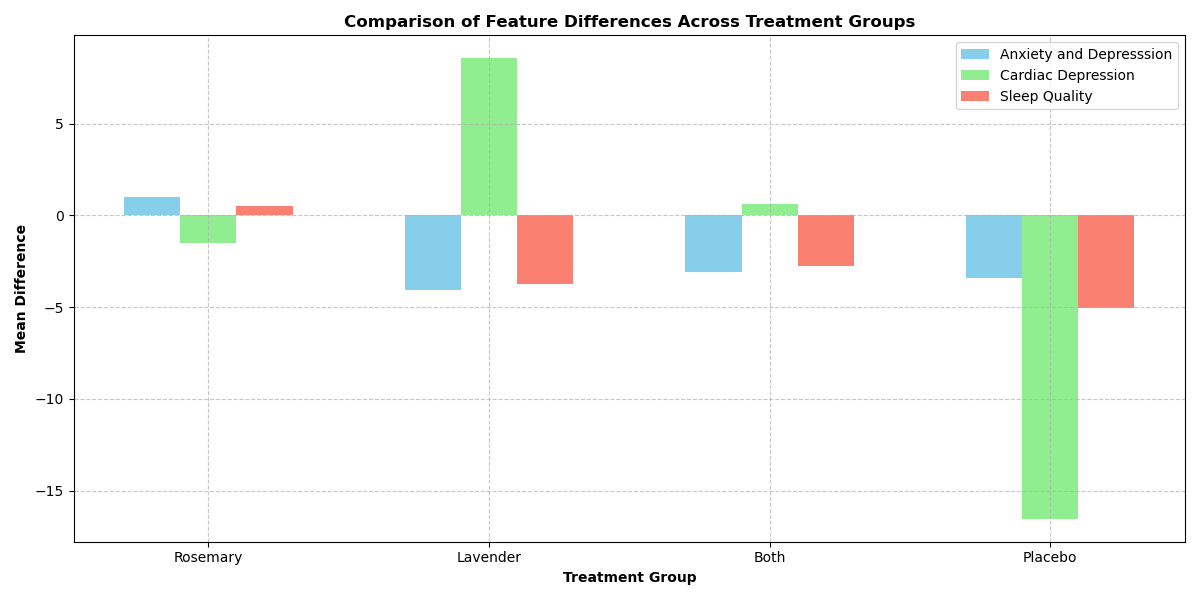
\includegraphics[width=\textwidth]{../figures/mean_feature_diffs.png}
    \caption{Mean Differences by Group for Survey Responses}
    \label{fig:mean_feat_diffs}
\end{figure}
Additionally, a table detailing the results of the t-tests ran is provided below.
\begin{table}[H]
\resizebox{\textwidth}{!}{%
\begin{tabular}{|c|c|c|c|c|}
\hline
         & Group 1       & Group 2       & Group 3       & Group 4       \\
\hline
\textbf{HADS\_diff} & t = 2.5480, p = 0.0164 & t = -6.0869, p = 0.0000 & t = -6.9402, p = 0.0000 & t = -6.7950, p = 0.0000 \\
\hline
\textbf{CDS\_diff}  & t = -3.1324, p = 0.0039 & t = 4.0203, p = 0.0003 & t = 0.4614, p = 0.6480 & t = -6.2800, p = 0.0000 \\
\hline
\textbf{PSQI\_diff} & t = 1.7873, p = 0.0843  & t = -8.8034, p = 0.0000 & t = -7.1297, p = 0.0000 & t = -10.1687, p = 0.0000 \\
\hline
\end{tabular}%
}
\caption{One-sample t-tests for HADS\_diff, CDS\_diff, and PSQI\_diff (horizontal format)}
\end{table}

Each of the ANOVAs ran were considered significant under any reasonable $\alpha$
(all p-values were $<1*10^{-8}$),
meaning the Tukey HSD was ran. For the HADS survey, group one was considered
significantly different from groups two, three and four, with no other groups
being considered significantly different.  For the CDS survey, every group
was considered significantly different from one another, except for groups
one and three. Finally, for the PSQI survey, all groups were significantly different from
one another, except for group two between groups three and four.
\newpage
\section{Discussion}
Revisiting the hypotheses that this study hoped to answer regarding aromatherapy
as a treatment for various types of mental-wellbeing measurements following
cardiac arrest, it can be
shown through the variety of statistical tests performed that there is a
significantly different outcome between the placebo group and any of the
experimental groups for one if not all of the features of interest. Additionally,
the estimated true differences between the placebo and the experimental groups
tended to be negative, indicating an overall improvement in mental well-being.
Thus, hypothesis one is demonstrated as plausible for the experimental groups,
for the HADS and PSQI survey, and the CDS survey for group four.  Additionally,
for hypotesis two, The effectiveness between groups is significantly different
in certain aspects as demonstrated by the Tukey HSD, with group four having
the largest significant improvement in all categories.  Finally, due to
group four being significantly different than groups two and three for
several of the features of interest, it is reasonable to believe there may
be interaction effects between Rosemary and Lavendar when used in conjuction.
It is important to note that this study may be limited due to the fact that
it is not completely controlled, and different lifestyle habits may have manifested
and been confounding over the course of the month in regards to the effects it
may have had on mental well-being. A proper future direction for this research
would be to perform this experiment in a completely controlled environment,
in order to account for any lifestyle differences amongst the groups.  Another
way would be to increase the sample sizes of each group, in an attempt to
limit the confounding effects as much as possible.
\hfill \break \hfill \break
A repository of all the code and supplementary materials is housed in
\url{https://github.com/otdossett/STA475_miniproject}.

\end{document}


